\documentclass[12pt]{article} 

\usepackage[latin1]{inputenc}
\usepackage[spanish]{babel}
\usepackage{color}
\usepackage{multicol}
\usepackage{amsmath}
\usepackage{amssymb}
\usepackage{enumerate}
\usepackage{graphics}
\usepackage{graphicx}

\title{STACKS}
\author{Sara Chica, Rodrigo Gualtero}
\date{15 de Diciembre, 2012}

\begin{document}
\maketitle
\tableofcontents

\section{Introducci�n}
Este es un problema de Timus, identificado con el c�digo \textit{1220}, en el cual se desea desarrollar un gestor de memoria el cual debe trabajar con una gran cantidad de pilas.
\section{Definici�n del problema}
Este problema busca almacenar varias pilas y en estas pilas almacenar diferentes valores.
\subsection{Entrada}
Primero entra un n�mero (n) que indica el n�mero total de operaciones.
\\Seguido a ello, entra n lineas, cada una indicando que operaci�n realizar, en que pila y que valor adicionar, en caso de ser "PUSH".
\\El n�mero de pilas no excede 1000; el de operaciones 100000 y el valor es menor a $10^{9}$.
\subsection{Salida}
Imprime cada uno de los valores que salen por la operaci�n "POP".
\section{Modelamiento matem�tico}
Una pila es ua estructura de datos, en la cual el acceso a sus datos es de tipo LIFO(Last In First Out), <<�ltimo en entrar, primero en salir>>; esta cuenta con dos operaciones principales:
\\Push: Agrega un objeto a la pila.
\\Pop: Elimina el �ltimo elemento de la pila.
\begin{center}
	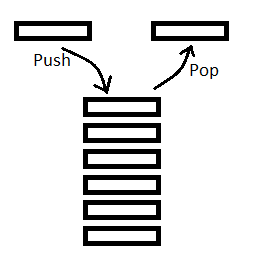
\includegraphics[height=0.50\textwidth]{pila.png}
	\\Imagen 1: Operaciones de la pila.
\end{center}
A continuaci�n se presenta un ejemplo de lo que es una pila y sus operaciones:
\begin{center}
	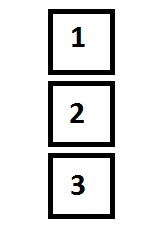
\includegraphics[height=0.50\textwidth]{1_2_3.png}
	\\Imagen 2: Pila original.
\end{center}
Si se desea adicionar a la pila anterior (Imagen 1) el valor 4; la pila quedar�a as�:
\begin{center}
	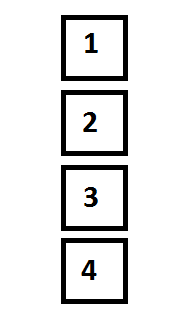
\includegraphics[height=0.50\textwidth]{1_2_3_4.png}
	\\Imagen 3: Pila con el valor 4.
\end{center}
\section{Planteamiento de la Soluci�n}
Para determinar la soluci�n a este problema es muy importante tener en cuenta el tiempo y la memoria que ocupar�a, debido a la gran cantidad de pilas y de operaciones.
\\Para ello es importante no crear todas las 1000 pilas, ya que puede que no sean tantas.
\\El problema se resuelve por medio de una estructura que permita contener cada una de las pilas, sin necesidad de saber su cantidad.
\section{Conclusiones}
\begin{enumerate}
	\item Es importante tener en cuenta el tiempo y la memoria que ocupa resolver el problema.
	\item Las pilas son usadas principalmente para implementar recursividad, evaluar expresiones en notaci�n postfija.
	\item Las pilas son bastante usadas debido a que son simples y tienen un ordenamiento impl�cito.
\end{enumerate}
\end{document}